\documentclass{beamer}
\usetheme[sectionpage=none]{metropolis}
% Theme settings
\setbeamerfont{footnote}{size=\tiny}

\usepackage[utf8]{inputenc}
\usepackage[T1]{fontenc}
\usepackage{textcomp}
\usepackage{babel}
\usepackage{amsmath, amssymb, mathtools}
\usepackage{listings}
\usepackage[ruled,vlined]{algorithm2e}

% % figure support
\usepackage{multimedia}
\usepackage{import}
\usepackage{xifthen}
\usepackage{pdfpages}
\usepackage{tikz}
\usepackage{pgfplots}
\pgfplotsset{compat=1.16}
\usepackage{transparent}
\usepackage{subcaption}

\usepackage[backend=biber]{biblatex}
\usepackage{csquotes}
\addbibresource{reference.bib}

\pdfsuppresswarningpagegroup=1

\title{
  A Variety of Approaches to \\
  the Nonuniform Fast Fourier Transform
}
\author{Kosuke Sugita and Connor Robertson}
\date{December 17, 2021}

\begin{document}
\frame{\titlepage}
% \frame{\tableofcontents}

% SECTIONS
%%%%%%%%%%%%%%%%%%%%%%%%%%%%%%%%%%%%%%%%%%%%%%%%%%%%%%%%%%%%%%%%%%%%%%%%%%%%%%%
\section{Introduction}
%%%%%%%%%%%%%%%%%%%%%%%%%%%%%%%%%%%%%%%%%%%%%%%%%%%%%%%%%%%%%%%%%%%%%%%%%%%%%%%
\begin{frame}
    \frametitle{Introduction}
    \textbf{Applications for NUFFT:}
    \begin{itemize}
        \item MRI Imaging - magnetic field reads frequency domain at nonuniform points
        \item Numerical solutions to PDEs - consider radial points or Chebyshev points to better resolve domain
        \item Coarse graining particles - Nonuniform distribution of discrete items to continuous field
    \end{itemize}

    \vfill

    Nonuniform samples: $(x_n, f(x_n))$:
    \begin{align*}
        \hat{f}(k) = \sum_{n=0}^{N-1} f(x_n) e^{-i x_n k} \approx \int_{-\infty}^{\infty} f(x) e^{-i x k}dx
    ,\end{align*}
    *\textit{Order $O(N^{2})$}
\end{frame}

\begin{frame}
  \frametitle{Concept}
  \textbf{Key idea:}
  \begin{enumerate}
      \item Need uniform points for FFT symmetry
      \item Use nonuniform points to cheaply sample uniform points
  \end{enumerate}

  \vfill

  \begin{columns}
      \begin{column}{.5\textwidth}
        \textbf{Approaches:}
        \begin{itemize}
            \item Interpolation
            \item Convolution of mollifier / window function
            \item Low rank approximation to DFT matrix
        \end{itemize}
      \end{column}
      \begin{column}{.5\textwidth}
        \centering 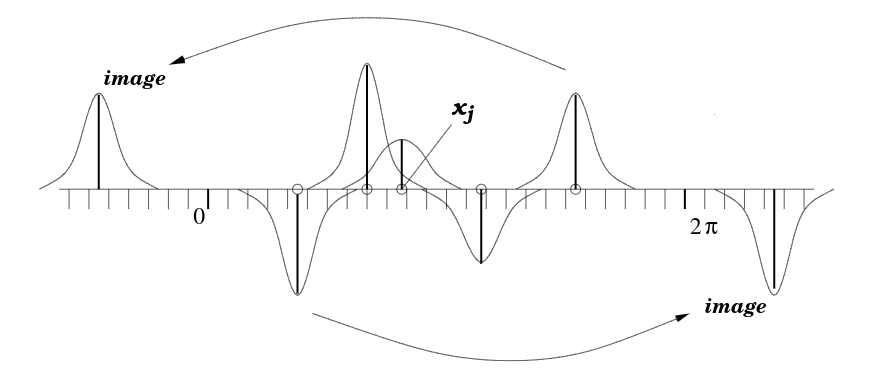
\includegraphics[width=\textwidth]{images/sample_gaussian.png}
      \end{column}
  \end{columns}
\end{frame}

\section{Numerical Examples}

\begin{frame}
  \frametitle{Sampling uniform points}
  Different sampling methods illustrated:

  \vfill

  \centering 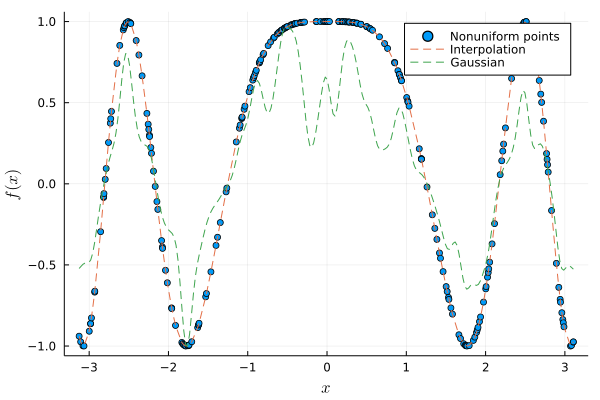
\includegraphics[width=.8\textwidth]{images/conv_vs_interp.png}
\end{frame}

\begin{frame}
  \frametitle{Comparison of methods output}
  Spectrum of results:

  \vfill

  \centering 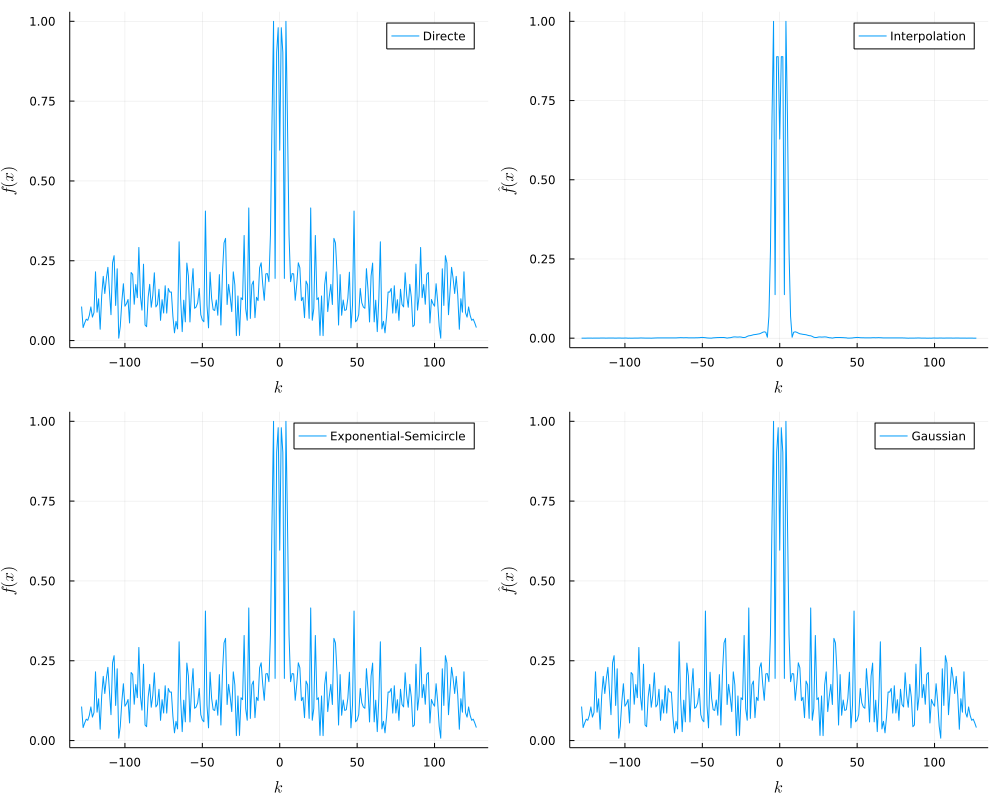
\includegraphics[width=.8\textwidth]{images/spectrum.png}

\end{frame}

\begin{frame}
  \frametitle{Speed}
  All methods scale far better than direct evaluation:

  \vfill

  \centering 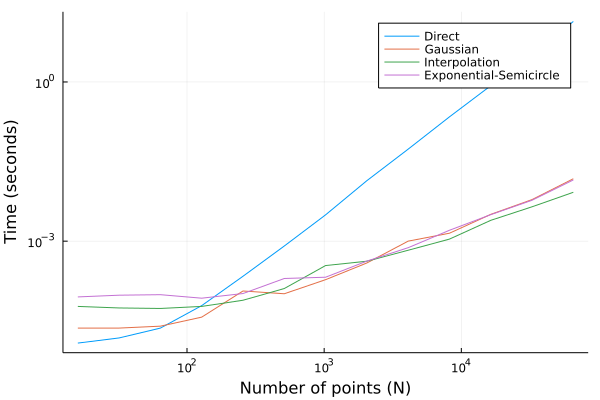
\includegraphics[width=.8\textwidth]{images/n_vs_time.png}

\end{frame}

\section{Conclusion}
\begin{frame}
  \frametitle{Conclusion}

  \begin{itemize}
      \item Sampling uniform points from nonuniform points is delicate - speed vs accuracy
      \item Selecting sampling method is an active research topic
      \item Alternative versions are appearing - low rank approximation
  \end{itemize}


\end{frame}
\end{document}
